% ============================================================
%  APPENDIX A — EXPERIMENT 1 FULL DETAILS
%  Place after the main body, e.g. \appendix\section{...}
% ============================================================

\section{Experiment 1: Prospective Forecast Updating}
\label{app:exp1}

Experiment~1 measures whether forecast revisions follow evidence direction and
whether directional packets produce larger changes than orthogonal packets.
All reported counts refer to parseable records in the frozen consistency report
unless stated otherwise.

\subsection{Study Design, Sample, and Agent Roster}
\label{app:exp1-sample}

\paragraph{Design at a glance.}
Experiment~1 crosses ten forecasting agents with a frozen set of unresolved binary
Polymarket questions.  The pipeline has four stages: (1)~freeze the market sample;
(2)~obtain one or more initial forecasts from each agent; (3)~generate nine synthetic
evidence packets for each of the 100 core markets (three pro-$H_1$, three
anti-$H_1$, and three causally orthogonal); and (4)~ask the same agent to revise each
parseable initial forecast after receiving one packet at a time.  The unit of analysis is an \emph{agent $\times$ market $\times$ initial run
$\times$ counterfactual packet} update.  Requested repeat
counts were five initial runs for frontier agents and three for local agents; realized
valid counts are uneven because of provider failures, parsing failures, and targeted
top-ups.  Section~\ref{app:metrics} specifies how those records are normalized and
aggregated.

\subsubsection{Sampling Frame and Market Selection}
\label{app:market-selection}

The primary sampling frame is a Polymarket API snapshot taken on June~9, 2026.
Selection was deterministic given that snapshot.  We retained markets that were
binary, active and unresolved, scheduled to resolve 14--180 days after sampling,
priced strictly between 0.10 and 0.90 on the YES contract, and supported by at least
\$1,000 in USD volume.  A keyword-based relevance filter retained politics,
government, elections, economics, technology, and geopolitics while excluding
sports, cryptocurrency, entertainment, and other out-of-scope topics.  When several
contracts belonged to the same event, we retained the highest-volume contract.

The recorded filter funnel makes the sampling loss explicit.  The snapshot contained
60,989 binary records; 37,386 were active, 8,639 passed the topic filter, 3,570 passed
the resolution-window filter, 1,403 passed the price filter, 839 passed the volume
filter, and event-level deduplication left 436 candidates.  A diversity pass selected
the 100-market core using a cosine-similarity threshold of 0.25 and a maximum of
16 markets per topical bucket.  The frozen core contains 16 global-election,
16 other, 15 Iran-nuclear, 12 U.S.-federal-policy, 10 AI/technology, 9 U.S.
state-election, 7 Russia--Ukraine, 5 Brazil, 5 U.S.-midterm, 3 macroeconomic,
and 2 China--Taiwan markets.

Counterfactual generation and Stage~3 updating use this 100-market core for every
model. Llama~3.1-70B has 99 analyzable markets because one market has no parseable
initial forecast.

\begin{center}
\begin{minipage}{\linewidth}
\centering
\captionof{table}{Representative markets from the frozen 100-market core.
Snapshot mid is the stored YES midpoint on June~9, 2026, not an eventual
outcome.}
\label{tab:markets}
\footnotesize
\resizebox{\linewidth}{!}{%
\begin{tabular}{llc}
\toprule
\textbf{Question} & \textbf{Topic} & \textbf{Snapshot mid} \\
\midrule
Will Renan Santos win the 2026 Brazilian presidential election? & Brazil & 0.17 \\
US--Iran nuclear deal by June~30? & Middle East & 0.20 \\
US $\times$ Iran permanent peace deal by July~31, 2026? & Iran & 0.32 \\
Will a new Gemini flagship be released by June~30, 2026? & AI/technology & 0.89 \\
\bottomrule
\end{tabular}%
}
\end{minipage}
\end{center}

\subsubsection{Agent Roster and Execution Modes}
\label{app:agent-roster}

The roster comprises three hosted frontier systems and seven open-weight local systems
(Table~\ref{tab:agent-roster}).  The hosted models ran through Azure AI~Foundry and used
its native search-supported Responses workflow \citep{microsoft2026foundry}.  Local
models were served by Ollama \citep{ollama2026} on cluster GPUs; their research turn was supplied by Tavily search.  All agents received the same substantive three-step contract: build an event
model, gather current evidence, and emit a structured forecast. Provider-specific
search orchestration and model runtimes were not identical.

\begin{center}
\begin{minipage}{\linewidth}
\centering
\captionof{table}{Experiment~1 agent roster and requested initial-forecast repeats.  Requested
$k$ is the collection target, not an analysis denominator; exact realized coverage
appears in Table~\ref{tab:model-summary}.}
\label{tab:agent-roster}
\small
\begin{tabular}{llllc}
\toprule
\textbf{Model} & \textbf{Runtime} & \textbf{Research search} &
\textbf{Nominal params} & \textbf{Requested $k$} \\
\midrule
GPT-5.4          & Azure Foundry & Foundry native & --- & 5 \\
Claude Opus~4.8  & Azure Foundry & Foundry native & --- & 5 \\
DeepSeek V4-Pro  & Azure Foundry & Foundry native & --- & 5 \\
Qwen~2.5-7B      & Ollama & Tavily & 7B  & 3 \\
Qwen~2.5-14B     & Ollama & Tavily & 14B & 3 \\
Qwen~2.5-32B     & Ollama & Tavily & 32B & 3 \\
Qwen~2.5-72B     & Ollama & Tavily & 72B & 3 \\
Llama~3.1-8B     & Ollama & Tavily & 8B  & 3 \\
Llama~3.1-70B    & Ollama & Tavily & 70B & 3 \\
Llama~3.3-70B    & Ollama & Tavily & 70B & 3 \\
\bottomrule
\end{tabular}
\end{minipage}
\end{center}

For local models, reasoning calls used the frozen configuration temperature of 0.1 and
the final JSON-formatting call used temperature 0.0.  Search queries, tool responses,
token counts, parse errors, and provider errors were retained with each run.  Some
smaller models returned probabilities on a 0--100 rather than 0--1 scale.  The
initial-forecast parser converted those values, but the frozen Stage~3 data retain a
mixed-scale Qwen~2.5-7B subset documented in
Section~\ref{app:record-processing}.

\subsection{Forecast, Intervention, and Validation Protocol}
\label{app:exp1-protocol}

\subsubsection{Initial Forecast Elicitation}
\label{app:prompts}

\paragraph{Design rationale.}
The elicitation asks each agent to restate the resolution criterion, construct
explicit YES and NO hypotheses, identify a status-quo trajectory, research
current evidence, and map its final YES probability to the posterior assigned to
$H_1$. Question restatement and status-quo anchoring follow prior
forecasting-prompt evidence \citep{halawi2024approaching,wilson2025automated}.

\paragraph{Executed three-turn sequence.}
Every frozen initial forecast followed the same substantive sequence, with
provider-specific tool plumbing:

\begin{enumerate}
  \item \textbf{Event model.}  The agent received the question, full resolution
        description, days to resolution, and category.  It restated what would count
        as YES versus NO; identified actors, mechanisms, and latent variables; formed
        $H_1$ (YES) and $H_2$ (NO); and described the status-quo outcome.
  \item \textbf{Current-evidence research.}  The agent gathered evidence for and
        against each hypothesis, checked whether the required chain of events was
        plausible within the remaining time, and revised its assessment.  Frontier
        systems used Azure Foundry's native search workflow; local systems generated
        queries that were executed through Tavily and received the returned evidence
        in context.
  \item \textbf{Structured forecast.}  A final call converted the accumulated analysis
        to the common JSON contract below.  A run entered downstream processing only
        when this object was parseable.
\end{enumerate}

The research turn included this calibration instruction:

\begin{small}
\begin{verbatim}
Given the days remaining, what chain of events is required for H1, and
is that pace of change plausible? Give extra weight to the status quo;
depart substantially only when concrete directional evidence warrants it.
\end{verbatim}
\end{small}

The common output contract was:

\begin{small}
\begin{verbatim}
{
  "event_model": {
    "key_actors": [str],
    "key_mechanisms": [str],
    "latent_variables": [str]
  },
  "hypotheses": [
    {"id": "H1", "description": str,
     "prior_probability": float, "posterior_probability": float,
     "supporting_evidence": [str], "contradicting_evidence": [str]},
    {"id": "H2", ...}
  ],
  "hypothesis_to_forecast_mapping": str,
  "yes_prob": float,
  "confidence": "low"|"medium"|"high",
  "rationale": str,
  "evidence_sources": [str]
}
\end{verbatim}
\end{small}

The contract makes the intended invariant explicit: \(\hat p=P(H_1)\).  The ICS
metric tests whether the returned fields obey that invariant after an intervention.
The substantive prompt contract was common, but prompts were not byte-identical across
runtimes because the hosted and local search interfaces require different orchestration.

\subsubsection{Counterfactual Packet Construction and Audit}
\label{app:cf-taxonomy}

For each of the 100 core markets, GPT-5.4 generated nine synthetic evidence packets:
three pro-$H_1$, three anti-$H_1$, and three orthogonal.  Each generation call received
the market question, resolution description, and a canonical parseable initial event
model and forecast.  It produced:

\begin{itemize}
  \item \textbf{evidence\_headline}: one sentence that states the new development;
  \item \textbf{evidence\_text}: a 2--4 sentence synthetic wire-style item;
  \item \textbf{mechanism\_targeted}: the causal pathway by which the item should
        affect, or remain irrelevant to, resolution;
  \item \textbf{direction}: \texttt{pro\_H1}, \texttt{anti\_H1}, or
        \texttt{orthogonal};
  \item \textbf{slot\_type}: one of the six roles in
        Table~\ref{tab:slot-taxonomy}; and
  \item \textbf{plausibility\_rating}: the generator's 1--5 self-rating.
\end{itemize}

Within each direction, sequential exclusion required a new packet to target a different
actor and mechanism from earlier packets.  Search was disabled so the packets remained
controlled synthetic premises rather than paraphrases of live reporting.

\begin{center}
\begin{minipage}{\linewidth}
\centering
\captionof{table}{Counterfactual slot taxonomy.  Each market receives one packet of every
direction--slot combination shown, for nine packets total.}
\label{tab:slot-taxonomy}
\small
\begin{tabular}{p{2.5cm} p{1.8cm} p{7.5cm}}
\toprule
\textbf{Slot type} & \textbf{Direction} & \textbf{Role in the intervention} \\
\midrule
DATA        & pro, anti & A measurement, price signal, statistic, or poll that
               shifts the likelihood of $H_1$. \\
DECISION    & pro, anti & An actor decision, official statement, policy announcement,
               commitment, or refusal bearing on $H_1$. \\
STRUCTURAL  & pro, anti & A technical, logistical, legal, or contextual change that
               makes $H_1$ more or less likely. \\
PROCEDURAL  & orthogonal & A same-domain administrative or process update without a
               direct causal path to $H_1$ versus $H_2$. \\
PERSONNEL   & orthogonal & A staffing or leadership change involving a relevant actor
               but an issue unrelated to $H_1$ versus $H_2$. \\
BACKDROP    & orthogonal & Contextual economic, logistical, or social information that
               sets the scene without shifting the outcome odds. \\
\bottomrule
\end{tabular}
\end{minipage}
\end{center}

\paragraph{Packet-level integrity checks.}
The frozen packet file contains 900/900 parseable records: 100 markets multiplied by
nine packets, with exactly 300 pro-$H_1$, 300 anti-$H_1$, and 300 orthogonal records.
Every packet has a nonempty headline, and the logs contain zero search calls.  All 900
generator-assigned plausibility ratings equal 4/5. That field documents the
generator's compliance claim but provides neither variation nor independent
validation; the separate human materials review is reported below.
These checks establish structural completeness, not that directional strength or
difficulty is perfectly matched across packets.

As an illustration, for the Hormuz market the pro-$H_1$ headline
\textit{Oman says Iran agrees daily protected windows for commercial Hormuz transits}
elicited the largest single update reported in the viewer: Claude Opus~4.8 revised
from 10\% to 45\% (\(\Delta\hat p=+35\)~pp).  The orthogonal IMO
incident-reporting item produced negligible movement.

\subsubsection{Stage~3 Update and Pairing}
\label{app:update-protocol}

Each packet was presented separately with the agent's own parseable initial structured
forecast.  The agent was instructed to accept that single synthetic development as true
for the exercise, identify whether it was already implicit in its background view, and
return the same structured forecast with revised $H_1$, $H_2$, and YES probabilities
plus a one-sentence \texttt{novelty\_assessment}.  Search was disabled, and agents were instructed to treat the intervention as
true without online verification.

For an agent--market cell with \(k\) parseable initial runs, the intended crossed design
contains \(9k\) update records.  Each update is conditionally independent in prompt
context: it contains one initial run and one packet, never another packet or another
agent's answer.  The novelty prompt was intended to discourage large revisions for
background information; novelty itself is not used as a reported endpoint and should
not be viewed as a validated correction.

Provider interruptions, parse failures, and subsequent top-ups make realized cells
uneven.  We therefore report exact valid record and market denominators by model in
Table~\ref{tab:model-summary} rather than treating requested \(k\) or the theoretical
\(9k\) as observed sample sizes.

\subsection{Estimands, Record Processing, and Aggregation}
\label{app:metrics}

\subsubsection{Record Construction, Deduplication, and Missingness}
\label{app:record-processing}

The frozen analysis artifact is
\path{exp1_prospective/data/results/consistency_report_2026-06-17.json}; tables in
this paper use its stored denominators rather than a fresh scan of the evolving
collection directories.  During report construction, date suffixes are stripped from
task identifiers so daily collection files join to the same market.  Counterfactuals
are deduplicated by \texttt{cf\_id}; updates are deduplicated by
\texttt{update\_id}, with a parseable record preferred over an error record when both
exist.  Files are read newest first for the initial-forecast and market-price lookup.
Malformed JSON lines are skipped.  Missing values are handled per estimand: a record
may therefore contribute to ICS but not EHC, or vice versa, depending on which fields
parse.

Stage~3 update fields were evaluated on their stored scale in the frozen report.
For Qwen~2.5-7B, 207 of 8,636 deduplicated records store
\texttt{updated\_yes\_prob} above 1.5; no other model does. Its directional sign
metrics remain usable, but its absolute revision magnitudes and sensitivity
ratio are scale-contaminated and are omitted from the paper tables.

\subsubsection{Consistency Estimands}
\label{app:metric-definitions}

For update record \(i\), let \(d_i\in\{+1,-1\}\) denote the intended direction
(\(+1\) for pro-$H_1$, \(-1\) for anti-$H_1$).  Orthogonal packets do not have an
intended sign and are excluded from EHC and HFC.  The 3~pp movement threshold excludes
cases in which a model effectively leaves the forecast unchanged.

\paragraph{Evidence--Hypothesis Consistency (EHC).}
Let \(\Delta p(H_1)_i=p(H_1)_i^{\mathrm{post}}-\hat p_i^{\mathrm{initial}}\).
For directional records with \(|\Delta p(H_1)_i|\geq0.03\),
\begin{equation}
  \mathrm{EHC}_i=\mathbf{1}\!\left[\Delta p(H_1)_i d_i>0\right].
  \label{eq:ehc}
\end{equation}
EHC asks whether the updated hypothesis field moves in the direction implied by the
packet; it does not score the size of that movement.

\paragraph{Hypothesis--Forecast Consistency (HFC).}
Let \(\Delta\hat p_i=\hat p_i^{\mathrm{post}}-\hat p_i^{\mathrm{initial}}\).
For directional records with \(|\Delta\hat p_i|\geq0.03\),
\begin{equation}
  \mathrm{HFC}_i=\mathbf{1}\!\left[\Delta\hat p_i d_i>0\right].
  \label{eq:hfc}
\end{equation}
HFC asks the same directional question of the headline YES probability.

\paragraph{Internal Coherence Score (ICS).}
ICS is defined whenever both updated fields parse and is unconditional on movement:
\begin{equation}
  \mathrm{ICS}_i=\mathbf{1}\!\left[
  \left|\hat p_i^{\mathrm{post}}-p(H_1)_i^{\mathrm{post}}\right|<0.02\right].
  \label{eq:ics}
\end{equation}
The inequality is strict: a discrepancy of exactly 2~pp does not pass.

\paragraph{Directional sensitivity.}
Packet selectivity is summarized by
\begin{equation}
  \mathrm{Sensitivity}=
  \frac{\overline{|\Delta\hat p|}_{\mathrm{pro}+\mathrm{anti}}}
       {\overline{|\Delta\hat p|}_{\mathrm{orthogonal}}}.
  \label{eq:sensitivity}
\end{equation}
A value near one indicates comparable movement for directional and orthogonal
packets; larger values indicate preferential response to directional packets. This
ratio is descriptive.  It cancels a uniform multiplicative scale within a model, but
does not repair mixed scales across records, hence the Qwen~2.5-7B caveat above.

\subsubsection{Aggregation and Uncertainty}
\label{app:aggregation}

For EHC, HFC, and ICS, the evaluator first pools eligible records within each
model--market cell to obtain a market-level rate.  The reported model score is the
unweighted mean of those market rates, so a market with more successful repeat runs
does not receive greater weight.  Reported standard errors are the sample standard
deviation of market-level rates divided by the square root of the number of markets.

Revision magnitudes and sensitivity use the deduplicated update records pooled
within model and direction. Their standard errors are record-level summaries and
do not model dependence among repeated initial runs or the nine packets from one
market; they should be read descriptively.

\subsubsection{Unconditional Directional Correctness and Threshold Robustness}
\label{app:exp1-threshold-robustness}

\paragraph{The two output fields are structurally coupled.}
The final-output schema explicitly instructs the agent that
$\hat p=P(H_1)$, and the Stage~3 prompt requests the same structure after
updating. EHC and HFC are therefore not independent tests of an inferred
hypothesis-to-forecast link. ICS is a schema-adherence diagnostic, while close
EHC--HFC agreement reflects a mixture of directional updating and compliance
with the prompted equality. Among the 26,010 relevant records with both updated
fields present, 25,984 (99.90\%) satisfy the equality exactly after scale
normalisation and 25,987 (99.91\%) satisfy it within the 2-pp ICS tolerance. We
therefore do not treat EHC--HFC parity as independent evidence for a latent
representation or for spontaneous propagation between separately elicited
quantities.

\paragraph{Unconditional estimand.}
For threshold $t$, Table~\ref{tab:exp1-threshold-robustness} retains a valid
directional update when $|\Delta|\geq t$ and reports the fraction for which
$d_i\Delta_i>0$. At $t=0$, every valid pro- and anti-$H_1$ update enters the
denominator and a zero change is scored incorrect. We first compute correctness
within market and then average markets equally, matching the primary analysis.
The \emph{Below 3 pp} column is the record-weighted fraction and count excluded
by the published 3-pp conditional metric. The table's $n$ is the complete
pre-threshold denominator: records require a parseable initial probability and
the applicable updated field, but are not selected on the direction or magnitude
of movement.

\begin{center}
\begin{minipage}{\linewidth}
\centering
\captionof{table}{Unconditional directional correctness and robustness to 0-,
1-, 3-, and 5-percentage-point movement thresholds. The 0-pp column is
unconditional over all valid directional updates and scores zero movement as
incorrect; positive-threshold columns condition on the stated magnitude.
\emph{Below 3 pp} gives the percentage and count omitted from the corresponding
published 3-pp EHC or HFC denominator. Rates are macro-averaged across markets.}
\label{tab:exp1-threshold-robustness}
\scriptsize
\setlength{\tabcolsep}{4pt}
\resizebox{\linewidth}{!}{%
% Generated by exp1_prospective/agent/evaluate_threshold_robustness.py
\begin{tabular}{llrrrrrr}
\toprule
& & & \multicolumn{4}{c}{Directional correctness} & \\
\cmidrule(lr){4-7}
\textbf{Model} & \textbf{Metric} & \textbf{$n$ valid} &
\textbf{0 pp} & \textbf{1 pp} & \textbf{3 pp} & \textbf{5 pp} &
\textbf{Below 3 pp} \\
\midrule
Claude Opus~4.8 & EHC & 2,119 & 98.2\% & 98.6\% & 99.0\% & 99.5\% & 18.1\% (383) \\
 & HFC & 2,119 & 98.3\% & 98.6\% & 99.0\% & 99.5\% & 18.1\% (383) \\
GPT-5.4 & EHC & 2,678 & 98.4\% & 98.4\% & 98.7\% & 98.8\% & 6.9\% (185) \\
 & HFC & 2,684 & 98.4\% & 98.4\% & 98.7\% & 98.8\% & 6.9\% (185) \\
DeepSeek V4-Pro & EHC & 2,929 & 97.3\% & 97.6\% & 97.7\% & 98.0\% & 12.7\% (371) \\
 & HFC & 2,929 & 97.3\% & 97.6\% & 97.7\% & 98.0\% & 12.6\% (370) \\
\midrule
Llama~3.3-70B & EHC & 1,788 & 96.4\% & 96.4\% & 96.5\% & 97.4\% & 0.7\% (12) \\
 & HFC & 1,788 & 96.4\% & 96.4\% & 96.5\% & 97.4\% & 0.7\% (12) \\
Llama~3.1-70B & EHC & 1,659 & 96.1\% & 96.1\% & 96.1\% & 96.7\% & 0.6\% (10) \\
 & HFC & 1,659 & 96.1\% & 96.1\% & 96.1\% & 96.7\% & 0.6\% (10) \\
Qwen~2.5-72B & EHC & 1,795 & 96.3\% & 96.3\% & 96.3\% & 96.4\% & 0.8\% (15) \\
 & HFC & 1,795 & 96.3\% & 96.3\% & 96.3\% & 96.4\% & 0.8\% (15) \\
Qwen~2.5-32B & EHC & 1,795 & 96.4\% & 96.4\% & 96.4\% & 96.5\% & 1.9\% (34) \\
 & HFC & 1,795 & 96.4\% & 96.4\% & 96.4\% & 96.5\% & 1.9\% (34) \\
Qwen~2.5-14B & EHC & 1,800 & 93.1\% & 94.4\% & 94.3\% & 94.3\% & 2.9\% (52) \\
 & HFC & 1,800 & 93.1\% & 94.4\% & 94.3\% & 94.3\% & 2.9\% (52) \\
Qwen~2.5-7B & EHC & 5,759 & 90.2\% & 90.2\% & 90.6\% & 90.8\% & 2.2\% (129) \\
 & HFC & 5,759 & 89.9\% & 90.2\% & 90.5\% & 90.8\% & 2.4\% (140) \\
Llama~3.1-8B & EHC & 3,601 & 88.1\% & 88.7\% & 88.7\% & 88.9\% & 1.7\% (62) \\
 & HFC & 3,604 & 88.4\% & 88.7\% & 88.7\% & 88.9\% & 1.4\% (52) \\
\bottomrule
\end{tabular}

}
\end{minipage}
\end{center}

\paragraph{Result.}
The threshold sweep preserves the qualitative conclusion but narrows its
wording. Frontier-model unconditional correctness is 97.3--98.4\%; at the
published 3-pp threshold it is 97.7--99.0\%. The 3-pp rule excludes 6.9\% of
GPT-5.4, 12.6--12.7\% of DeepSeek V4-Pro, and 18.1\% of Claude Opus~4.8
directional updates. Thus, the near-1.0 EHC/HFC values do not result from
discarding a majority of cases, and the conclusion is stable across 0, 1, 3,
and 5~pp. The precise statement is nonetheless \emph{99\% directionally correct
among updates of at least 3~pp}, not \emph{99\% coherent updating}. Small local
models have fewer sub-3-pp updates (0.6--2.9\%) but lower unconditional
correctness (88.1--96.4\%), so their errors are not hidden primarily by the
movement filter.

\paragraph{Normalisation and reproducibility.}
Before recomputing deltas, the analysis independently normalises the initial
headline probability, updated headline probability, and updated $H_1$
posterior from the documented $[0,1]$ or $[0,100]$ formats. This matters for
166 relevant Llama~3.1-8B records in which $H_1$ was emitted as a percentage
while \texttt{yes\_prob} was emitted as a proportion. The complete eligible
record and market counts at every threshold, invalid-field counts, market-level
standard errors, input-file SHA-256 hashes, and full-precision estimates are in
\path{exp1_prospective/data/results/threshold_robustness.json}. The table is
regenerated by
\path{exp1_prospective/agent/evaluate_threshold_robustness.py}; neither script
nor table uses outcomes or post-hoc item filtering.

\subsection{Extended Results}
\label{app:extended-results}

\subsubsection{Analysis Coverage}
Table~\ref{tab:model-summary} gives the exact Stage~3 record and market counts.
All models use the same 100-market core; Llama~3.1-70B has 99 analyzable markets
because one market has no parseable initial forecast.

\begin{center}
\begin{minipage}{\linewidth}
\centering
\captionof{table}{Valid Stage~3 update records and represented core markets by
agent.}
\label{tab:model-summary}
\small
\begin{tabular}{llrr}
\toprule
\textbf{Model} & \textbf{Type} & \textbf{Records} & \textbf{Markets} \\
\midrule
Claude Opus~4.8 & Frontier  & 3{,}125 & 100 \\
GPT-5.4         & Frontier  & 3{,}913 & 100 \\
DeepSeek V4-Pro & Frontier  & 4{,}395 & 100 \\
Llama~3.3-70B   & Local 70B & 2{,}682 & 100 \\
Llama~3.1-70B   & Local 70B & 2{,}490 &  99 \\
Qwen~2.5-72B    & Local 72B & 2{,}692 & 100 \\
Qwen~2.5-32B    & Local 32B & 2{,}693 & 100 \\
Qwen~2.5-14B    & Local 14B & 2{,}700 & 100 \\
Qwen~2.5-7B     & Local 7B  & 8{,}636 & 100 \\
Llama~3.1-8B    & Local 8B  & 5{,}404 & 100 \\
\midrule
\textbf{Total}  &           & \textbf{38{,}730} & \\
\bottomrule
\end{tabular}
\end{minipage}
\end{center}

\subsubsection{Revision Magnitudes and Packet Selectivity}
Table~\ref{tab:anchoring} reports mean absolute forecast revision
\(\overline{|\Delta\hat p|}\) by packet direction.  For the nine models whose updates
are consistently stored on 0--1, frontier systems show a clear separation between
directional and orthogonal packets, while local systems show weaker separation.

Qwen~2.5-7B has mixed 0--1 and 0--100 stored updates
(Section~\ref{app:record-processing}); we therefore omit its absolute magnitudes
and sensitivity ratio rather than present them as comparable estimates.

\begin{center}
\begin{minipage}{\linewidth}
\centering
\captionof{table}{Mean absolute forecast revision by counterfactual direction.
Sensitivity is mean directional divided by mean orthogonal movement; \(n\) is the
valid Stage~3 record count. Values are percentage points for models with
consistently stored 0--1 updates.}
\label{tab:anchoring}
\small
\begin{tabular}{llccccc}
\toprule
\textbf{Model} & \textbf{Type} & pro-$H_1$ & anti-$H_1$ & orthogonal
  & \textbf{Sensitivity} & $n$ \\
\midrule
Claude Opus~4.8 & Frontier  & 12.7\,pp & 9.6\,pp  & 0.5\,pp & $24.0\times$ & 3{,}125 \\
DeepSeek V4-Pro & Frontier  & 13.9\,pp & 11.4\,pp & 1.4\,pp & $8.9\times$  & 4{,}395 \\
GPT-5.4         & Frontier  & 10.6\,pp & 8.5\,pp  & 1.2\,pp & $8.2\times$  & 3{,}913 \\
\midrule
Llama~3.3-70B   & Local 70B & 14.8\,pp & 14.3\,pp & 2.3\,pp & $6.4\times$  & 2{,}682 \\
Llama~3.1-70B   & Local 70B & 14.8\,pp & 15.5\,pp & 3.3\,pp & $4.6\times$  & 2{,}490 \\
Qwen~2.5-72B    & Local 72B & 15.0\,pp & 10.2\,pp & 3.0\,pp & $4.2\times$  & 2{,}692 \\
Qwen~2.5-32B    & Local 32B & 15.0\,pp & 10.3\,pp & 4.0\,pp & $3.2\times$  & 2{,}693 \\
Qwen~2.5-14B    & Local 14B & 14.8\,pp &  8.6\,pp & 4.1\,pp & $2.9\times$  & 2{,}700 \\
Qwen~2.5-7B     & Local 7B  & --- & --- & --- & --- & 8{,}636 \\
Llama~3.1-8B    & Local 8B  & 11.1\,pp & 12.0\,pp & 5.9\,pp & $1.9\times$ & 5{,}404 \\
\bottomrule
\end{tabular}
\end{minipage}
\end{center}
Qwen~2.5-7B magnitude cells are omitted because 207 deduplicated updates are
stored above 1.5, mixing probability scales within the row.
Table~\ref{tab:anchoring} establishes the magnitude contrast; Figure~\ref{fig:causal-coherent} then places directional consistency and packet selectivity on a common visual scale.

\begin{center}
\begin{minipage}{\linewidth}
\centering
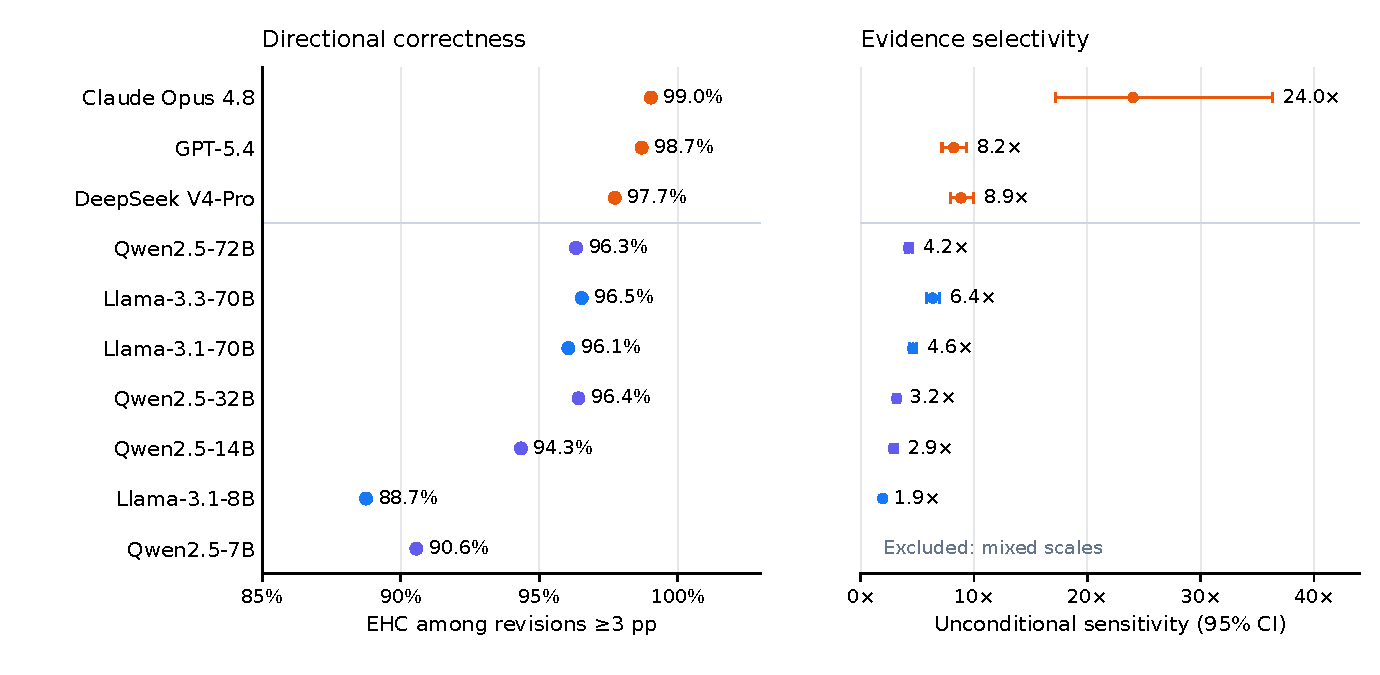
\includegraphics[width=\linewidth]{figures/exp1_ehc_sensitivity_combined.pdf}
\captionof{figure}{\textbf{Directional consistency and packet selectivity generally rise with
model scale.} \emph{Left:} EHC rises from $87$--$90\%$ for 7--8B local models to
roughly $98$--$99\%$ for frontier systems. \emph{Right:} sensitivity reaches
$1.9$--$6.4\times$ for local models and $8.2$--$24.0\times$ for frontier systems;
Qwen~2.5-7B is omitted from this panel because its archived absolute revisions mix
0--1 and 0--100 scales and therefore do not yield a comparable ratio.}
\label{fig:causal-coherent}
\end{minipage}
\end{center}






\subsection{Study Limits and Follow-up Analyses}
\label{app:exp1-limitations}

Five limits affect different claims: sample and outcome coverage,
counterfactual construct validity, prompt and runtime confounding, scale and
dependence, and the premise-acceptance instruction at Stage~3.

\subsubsection{Sampling and Outcome Scope}
The sample is a filtered slice of liquid, medium-horizon Polymarket questions,
not a probability sample of forecasting tasks. Topic exclusions, the
0.10--0.90 price window, the 14--180 day horizon, event deduplication, and the
diversity cap shape its difficulty distribution. Experiment~1 evaluates
conditional updating on unresolved questions; Experiment~4 separately evaluates
accuracy on resolved historical markets.

\subsubsection{Counterfactual Construct Validity}
The intervention audit establishes structural completeness, but not equal
difficulty. A single generator created all packets from a canonical initial
event model, and its automated plausibility score was uniformly 4/5. Direct
headlines can also permit a semantic sign classifier to pass without following
the intended causal path. The reported result therefore establishes
direction- and relevance-sensitive updating under semantically direct packets;
it does not establish mechanism-conditioned causal composition by itself.

We froze an initial seven-reviewer human materials protocol before registered
collection. It samples one report from each of 18 distinct markets, balanced
across six pro-YES, six anti-YES, and six orthogonal packets. Two later roster
extensions, made after interim responses were inspected, added independently
ordered assignments for R8 and R9 without changing the items or any earlier
assignment; we report the resulting
nine-reviewer roster as a sensitivity extension. Each reviewer rates all 18
items. Before the synthetic report, every item shows the market question,
resolution criteria, and matching summary from the frozen June~10 initial
forecast. The consent screen and every item instruct reviewers to treat
June~10, 2026 as the current date, use no later information, and not search the
web or consult an AI assistant. Intended directions, source IDs, generator
metadata, and model responses remain hidden.

Reviewers record the report's conditional direction, confidence, clarity,
real-world plausibility, and usability as an explicit hypothetical premise. The
frozen seven-reviewer item gate allowed one dissent: at least six reviewers had
to select the registered direction and mark the premise usable, median
confidence and clarity had to be at least 4/5, and median plausibility at least
3/5. The nine-reviewer extension uses the corresponding eight-of-nine rule. The
packet-level gate requires at least 15 of 18 items to pass and Fleiss'
$\kappa\geq .70$ for conditional direction. Ambiguous judgments remain in every
denominator.

A self-review conducted before registered collection removed three non-gating
questions---semantic directness, source verification, and optional free
text---and added the frozen June~10 background summary to every item. Practice
responses are stored separately and cannot enter the registered analysis.

In the August~22 analysis snapshot, seven reviewers had completed all 18 items.
The post-collection response-pattern rule described below excludes R2, leaving six
completed, quality-eligible reviewers (R1, R3--R6, and R9). R7 had submitted two
items and R8 had consented but submitted none, so the final nine-reviewer gate is
not yet available. Table~\ref{tab:stage3-human} reports the six-reviewer
snapshot. Exact-direction agreement is 81/108 (75.0\%); every included reviewer
exceeds a conservative $1/3$ directional-guessing baseline in a one-sided exact
binomial comparison (all unadjusted $p<.05$). We use $1/3$ rather than the form's
four-option $1/4$ baseline because the registered answer takes one of three
non-ambiguous directions. The task requires reviewers to integrate unfamiliar
market-specific background with a stipulated synthetic report and distinguish
directional, null, and ambiguous updates.

\paragraph{The six-reviewer snapshot does not meet the gate.} Applying the full
gate---including premise usability---to the six quality-eligible completed
reviewers retains 6 of 18 items. Considering direction alone, nine items draw at
most one dissent and five are unanimous. Fleiss' $\kappa$ for conditional direction is $.447$ over the four
response options ($.502$ if \emph{ambiguous} is folded into the null category), and
mean pairwise Cohen's $\kappa$ is $.452$ (range $.092$ to $.838$). These values
remain below the packet-level thresholds of 15 retained items and
$\kappa\geq.70$. Because the roster is incomplete, this is an interim diagnostic,
not a final gate decision, and it does not certify individual packets. The pooled
signal is stronger: the majority reviewer label matches the registered direction
on 16 of 18 items ($\kappa=.842$), and per-class exact agreement is 25/36 for
pro-$H_1$, 28/36 for anti-$H_1$, and 28/36 for orthogonal packets.
\begin{table}[t]
\centering
\small
\caption{\textbf{Stage~3 human materials judgments, six-reviewer snapshot.}
Direction is exact agreement with the registered conditional direction and
$\kappa$ is Cohen's $\kappa$ against that key over the four response options.
Confidence, clarity, and plausibility (C/C/P) are reviewer-level medians on 1--5
scales. The pooled row is descriptive because reviewers rated the same items; the
majority row takes the modal label per item, resolving ties to \emph{ambiguous}.}
\label{tab:stage3-human}
\begin{tabular}{lccccc}
\toprule
Reviewer & Direction agreement & $\kappa$ vs. key & $p$ vs. $1/3$ & Premise usable & C/C/P \\
\midrule
R1 & 12/18 (66.7\%) & .54 & .0039 & 10/18 & 4/4/4 \\
R3 & 12/18 (66.7\%) & .51 & .0039 & 13/18 & 4/4/3 \\
R4 & 18/18 (100.0\%) & 1.00 & $<.0001$ & 18/18 & 5/5/5 \\
R5 & 10/18 (55.6\%) & .38 & .0433 & 18/18 & 4/4/4 \\
R6 & 13/18 (72.2\%) & .61 & .0009 & 12/18 & 4/4/5 \\
R9 & 16/18 (88.9\%) & .84 & $<.0001$ & 18/18 & 5/5/5 \\
\midrule
Pooled & 81/108 (75.0\%) & --- & --- & 89/108 & --- \\
Majority label & 16/18 (88.9\%) & .84 & --- & --- & --- \\
\bottomrule
\end{tabular}
\end{table}

\begin{table}[p]
\centering
\scriptsize
\setlength{\tabcolsep}{3pt}
\caption{\textbf{Item-level Stage~3 materials audit for the six-reviewer snapshot.}
Key is the registered conditional direction; Majority is the modal panel response,
with ties assigned to \emph{ambiguous}. Agree and Usable give counts out of six;
C/L/P gives median direction confidence, clarity, and plausibility on 1--5 scales.
The interim item gate requires at least 5/6 registered-direction judgments, at
least 5/6 usable-premise judgments, median confidence and clarity of at least 4,
and median plausibility of at least 3. Failure codes identify the unmet criterion:
D (direction), C (confidence), L (clarity), P (plausibility), or U (premise
usability). Item numbers follow the frozen public packet order.}
\label{tab:stage3-items}
\begin{tabular}{@{}p{.38\linewidth}llcccc@{}}
\toprule
Question & Key & Majority & Agree & C/L/P & Usable & Gate \\
\midrule
1. Hormuz traffic normal by July 31 & More & More & 6/6 & 4.5/5/5 & 6/6 & Pass \\
2. Iran reaches World Cup knockouts & Less & Less & 4/6 & 4.5/5/4.5 & 5/6 & Fail (D) \\
3. Israel strikes Yemen by June 30 & No effect & No effect & 6/6 & 4.5/4/4.5 & 4/6 & Fail (U) \\
4. Netanyahu exits election by July 31 & More & More & 4/6 & 4.5/5/4.5 & 6/6 & Fail (D) \\
5. Anthropic valuation reaches \$1.1T & Less & Less & 5/6 & 4.5/4.5/5 & 6/6 & Pass \\
6. Oladokun starts Chiefs Week 1 & No effect & No effect & 5/6 & 4/4/3.5 & 5/6 & Pass \\
7. S\&P 500 reaches 7,700 in June & More & Ambig. & 3/6 & 4/4/5 & 6/6 & Fail (D) \\
8. Trump unfreezes Iranian assets & Less & Less & 5/6 & 4/4/4 & 5/6 & Pass \\
9. May durable-goods orders: 0--2\% & No effect & No effect & 3/6 & 3/3/3.5 & 4/6 & Fail (D,C,L,U) \\
10. China Q2 growth: 4.6--4.9\% & More & Ambig. & 2/6 & 3/3.5/4 & 3/6 & Fail (D,C,L,U) \\
11. Eisenkot joins Bennett--Lapid alliance & Less & Less & 4/6 & 4/5/5 & 5/6 & Fail (D) \\
12. Russia enters Orikhiv by July 31 & No effect & No effect & 6/6 & 5/3.5/4.5 & 4/6 & Fail (L,U) \\
13. Romanian PM is independent/technocrat & More & More & 4/6 & 4/4/4.5 & 6/6 & Fail (D) \\
14. Russia captures Kostyantynivka & Less & Less & 4/6 & 3/4.5/5 & 5/6 & Fail (D,C) \\
15. At least four June ChatGPT outages & No effect & No effect & 3/6 & 3/3.5/4.5 & 5/6 & Fail (D,C,L) \\
16. El-Sayed wins Michigan primary & More & More & 6/6 & 5/5/5 & 6/6 & Pass \\
17. Little is MN-02 Democratic nominee & Less & Less & 6/6 & 4.5/5/4 & 5/6 & Pass \\
18. OpenAI IPO close: \$1.25--1.5T & No effect & No effect & 5/6 & 4/3/4 & 3/6 & Fail (L,U) \\
\bottomrule
\end{tabular}

\end{table}

\paragraph{Models agree with the key more closely than reviewers do.} Scoring each
model's own updates on these same 18 packets---mean signed revision per packet,
thresholded at the same 3~pp used for EHC and HFC---gives
Table~\ref{tab:stage3-model-agreement}. The nine models with complete coverage
reach $\kappa=.67$ to $.92$ against the registered key, against a reviewer average of
$.65$, and $\kappa=.53$ to $.84$ against the human majority label. Claude Opus~4.8
is shown on the 12 packets for which it returned a parseable revision; the remaining
six carry empty records and are reported in the missingness appendix. Under these instructions, models match the key more closely than reviewers do.
This is not independent evidence for the materials, since the same directional
design generated both the packets and the registered key.


\begin{table}[t]
\centering
\small
\caption{\textbf{Model agreement on the same 18 Stage~3 packets.} A model's
direction label is its mean signed revision for that packet, thresholded at the
$3$~pp used for EHC and HFC. $\kappa$ is Cohen's $\kappa$ over the four response
options, taken against the registered key and against the majority reviewer label.
Claude Opus~4.8 covers 12 of 18 packets. Regenerate with
\protect\path{exp1_prospective/stage3_materials_annotation/compute_agreement.py}.}
\label{tab:stage3-model-agreement}
% Generated by stage3_materials_annotation/compute_agreement.py -- do not hand-edit.
\begin{tabular}{lccc}
\toprule
Model & $\kappa$ vs.\ key & Exact vs.\ key & $\kappa$ vs.\ human majority \\
\midrule
GPT-5.4 & 0.92 & 94.4\% & 0.84 \\
Llama~3.3-70B & 0.92 & 94.4\% & 0.76 \\
DeepSeek V4-Pro & 0.83 & 88.9\% & 0.76 \\
Llama~3.1-70B & 0.83 & 88.9\% & 0.69 \\
Qwen~2.5-72B & 0.83 & 88.9\% & 0.69 \\
Claude Opus~4.8 (12/18) & 0.75 & 83.3\% & 0.64 \\
Qwen~2.5-7B & 0.75 & 83.3\% & 0.60 \\
Llama~3.1-8B & 0.67 & 77.8\% & 0.53 \\
Qwen~2.5-14B & 0.67 & 77.8\% & 0.53 \\
Qwen~2.5-32B & 0.67 & 77.8\% & 0.53 \\
\bottomrule
\end{tabular}

\end{table}

After inspecting the first four completed submissions, we excluded one completed
reviewer (R2) for task misunderstanding: the reviewer selected \emph{more
likely} on 17 of 18 balanced items, including all six registered negative items
and five of six registered null items. This is a disclosed post-collection
deviation from the frozen no-exclusion rule. We applied the resulting quality
rule uniformly: exclude any completed reviewer who selects one direction on at
least 17 of 18 items. Raw responses are retained, and no item is removed or
relabeled. As a sensitivity tally, retaining R2 gives 88/126 (69.8\%) exact
agreement across the seven completed reviewers.

A post-task debrief occurred after R2 had seen their score and response pattern.
R2 reported interpreting the task as asking whether reports supported YES,
difficulty with English and market-specific terms, use of a dictionary and an
AI assistant despite the instruction, and reduced attention. We accepted no
re-rating and treat the debrief as context; the exclusion uses only the uniform
response-pattern rule.


The task requests no identifying or sensitive information. Under the authors'
institutional guidelines, this materials-review activity does not constitute
human-subjects research; consequently, no IRB review was sought.

Figure~\ref{fig:exp1-review-interface} records the reviewer-facing workflow. The
capture script at
\path{exp1_prospective/stage3_materials_annotation/capture_review_screenshots.py}
loads the frozen item packet against an empty temporary annotation database.
Later reviewer assignments changed access codes and item order only.


\begin{figure}[p]
\centering
\begin{subfigure}[t]{0.36\linewidth}
  \centering
  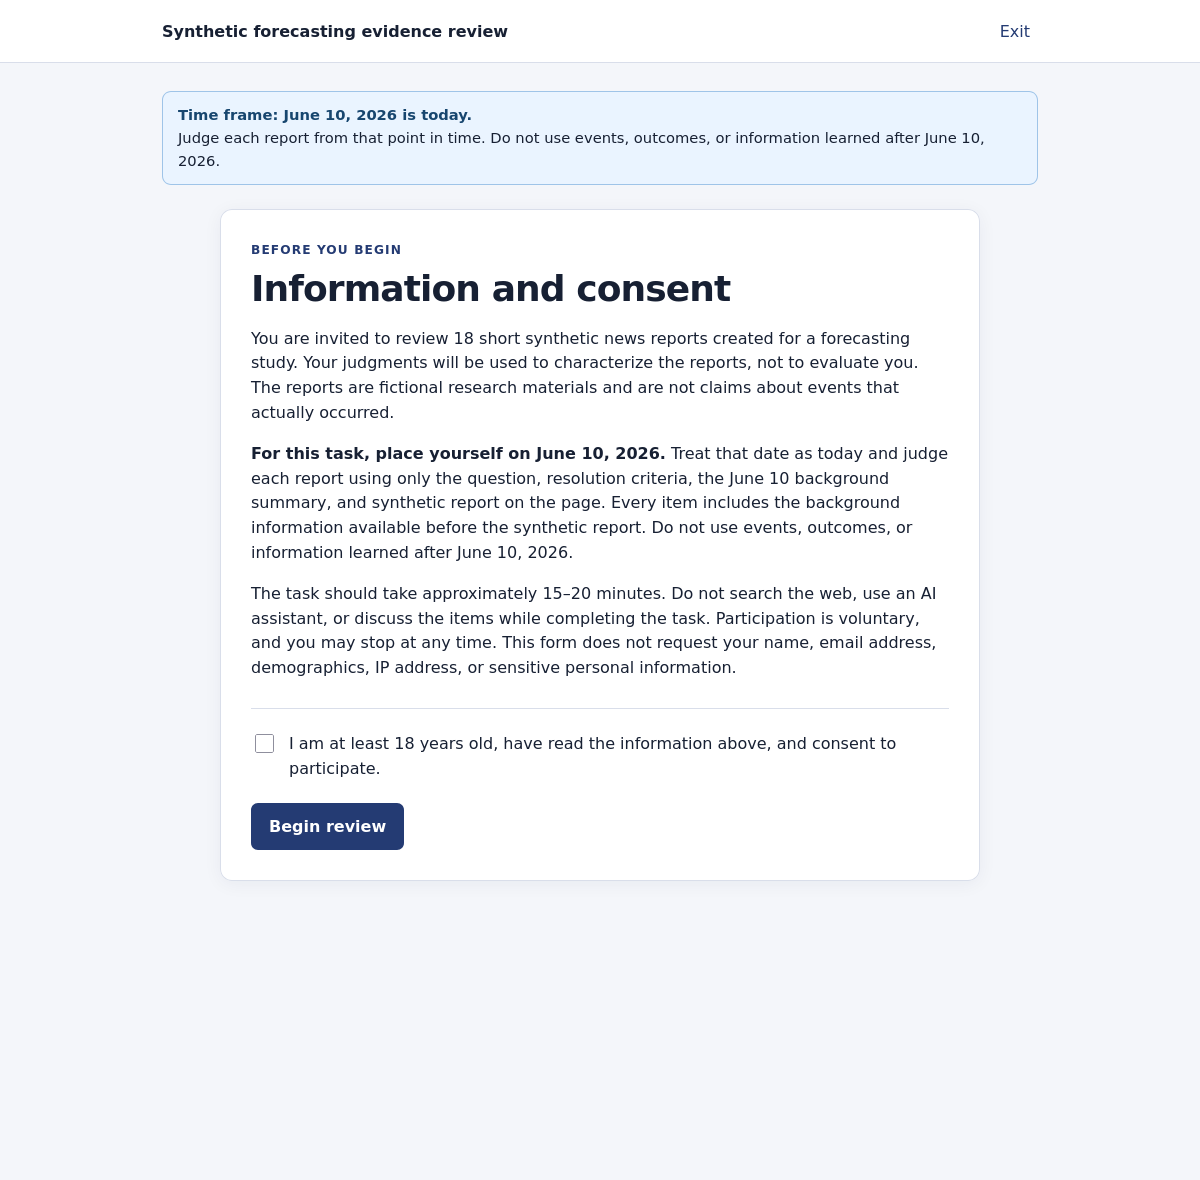
\includegraphics[width=\linewidth]{figures/exp1_stage3_review_consent.png}
  \caption{Information, temporal frame, and consent.}
\end{subfigure}\hfill
\begin{subfigure}[t]{0.60\linewidth}
  \centering
  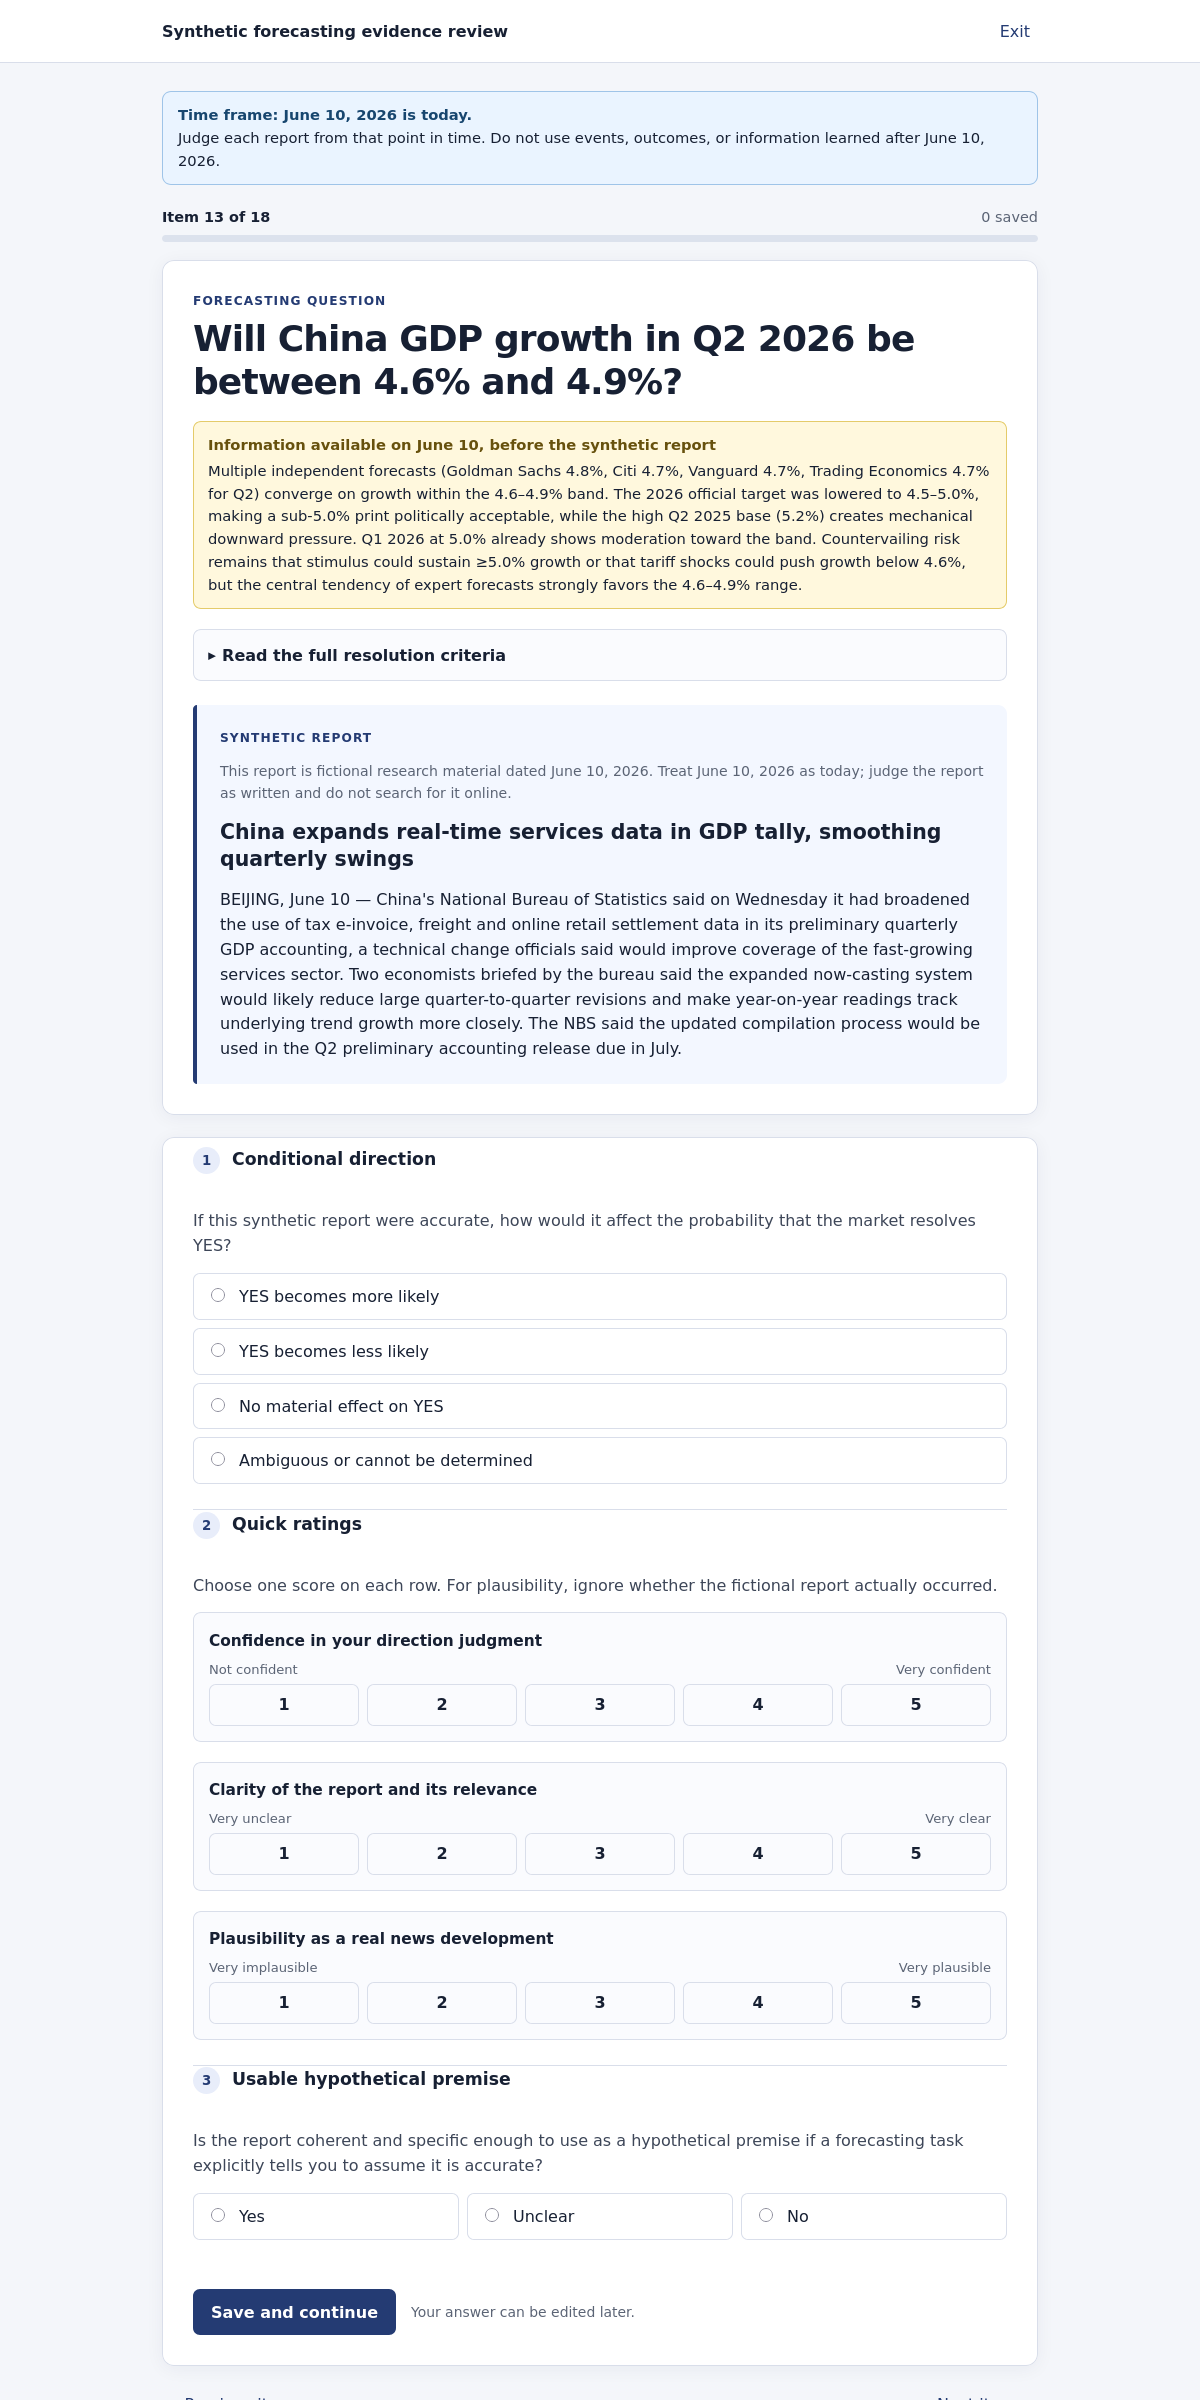
\includegraphics[width=\linewidth]{figures/exp1_stage3_review_item.png}
  \caption{A complete item with June~10 context, synthetic report, and five judgments.}
\end{subfigure}
\caption{\textbf{Stage~3 materials-review interface.} Reviewers enter a private
code before seeing the information-and-consent screen. Each item repeats the
June~10 temporal frame, presents the question and pre-report background, labels
the fictional evidence as a synthetic report, and collects conditional
direction, confidence, clarity, plausibility, and premise usability. Later
reviewer assignments changed access codes and item order only. Intended
direction and private packet metadata are hidden.}
\label{fig:exp1-review-interface}
\end{figure}

Orthogonal packets are a useful causal-irrelevance control, but are not equivalent to
receiving no new text.  A literal no-information update condition would separate
generic prompt-induced revision from response to topically adjacent content.  The very
small frontier orthogonal revisions (0.5--1.4~pp) are reassuring but do not replace
that control.

\subsubsection{Prompt, Retrieval, and Runtime Confounding}
Agents shared a substantive task contract, not byte-identical execution. Hosted
models used Azure Foundry search, while local models used Tavily results in an
Ollama workflow; temperatures and provider behavior also differ. Frontier--local
gaps therefore combine model capability with retrieval and runtime differences.

\subsubsection{Scale, Missingness, and Dependence}
Realized repeat counts are uneven because failures and top-ups differ by provider.
Equal-weight market aggregation prevents high-coverage markets from dominating EHC,
HFC, and ICS, but record-level revision summaries still treat repeated runs and packets
as independent.  Clustered or hierarchical uncertainty would be preferable.  The
mixed-scale Qwen~2.5-7B updates described in
Section~\ref{app:record-processing} additionally invalidate a clean magnitude
comparison for that row; a future frozen rerun should normalize every structured field
before deltas are written.

\subsubsection{Premise Acceptance at Stage~3}
Search is intentionally unavailable during updating, and agents are told to accept the
synthetic headline as true.  This isolates conditional updating but does not test source
verification or epistemic refusal.  A search-enabled condition might appropriately
decline to update on an unverifiable report, lowering EHC/HFC without implying less
inductive reasoning. The human materials review above uses the same conditional
premise instruction and therefore assesses comprehension and usability, not
source credibility. Both premise-acceptance and source-verification conditions
are needed to distinguish these behaviors.

\subsection{Reproducibility and Artifact Map}
\label{app:fig-code}

The paper treats the June~17 report as the frozen numerical authority.  The relevant
pipeline artifacts are:

\begin{itemize}
  \item \textbf{Sampling:}
        \path{exp1_prospective/fetch_markets/select_markets.py} and the June~9
        selection/diversity JSON and manifests in
        \path{exp1_prospective/data/selected_markets/}.
  \item \textbf{Initial elicitation:}
        \path{exp1_prospective/agent/forecast_agent.py} for hosted runs and
        \path{exp1_prospective/agent/run_local_forecast.py} for Ollama runs, with
        records and manifests in \path{exp1_prospective/data/initial_forecasts/}.
  \item \textbf{Interventions:}
        \path{exp1_prospective/agent/build_counterfactuals.py} and the frozen
        \path{exp1_prospective/data/counterfactuals/counterfactuals_2026-06-10.jsonl}.
  \item \textbf{Updates:}
        hosted and local update runners under \path{exp1_prospective/agent/}, with
        update records in \path{exp1_prospective/data/updated_forecasts/}.
  \item \textbf{Evaluation:}
        \path{exp1_prospective/agent/evaluate_consistency.py} and
        \path{exp1_prospective/data/results/consistency_report_2026-06-17.json}.
  \item \textbf{Human materials review:}
        the frozen protocol, blinded packet, browser application, tests, and
        analysis script in
        \path{exp1_prospective/stage3_materials_annotation/}.
  \item \textbf{Figures:}
        \path{paper/generate_figures.py} writes the direction-selective panel;
        \path{paper/generate_paper_figures.py} writes the combined
        EHC/sensitivity panel.
\end{itemize}

The model-update tables are defined by the June~17 frozen JSON. The mutable collection
directories contain later records, so evaluating their present contents would
define a different dataset. Bit-for-bit reconstruction begins from the frozen
JSON; a full pipeline reconstruction uses only the manifests and records included
in that freeze.

\clearpage
